\section{Firebase Cloud Messaging}
Duels are interactive by definition. A user \texttt{A} can dare another user \texttt{B} at any time as well as \texttt{B} can complete a round at any time. An application forcing users to manually check for updates (the so called \textit{polling}) would probably occur in a bad user experience. A smarter approach is known as \textit{push notification}. Our server sends out different messages for different situations. Clients (i.e. the app) needs only to be listening for news. The users are notified about new duel dares, new rounds available and duels completion. Tapping on those notification result, of course, in QuizFight opening the appropriate Activity. 

A key issue is actually implements from scratch this protocol. Some challenges would be the following:
\begin{itemize}
	\item How many times per second should the app check for updates?
	\item How should we identify a particular installation?
	\item How should we deal with new installations on different user's devices?
\end{itemize}

We then rely on a third-part well-known messaging protocol completely integrated with Google: \textbf{Firebase Cloud Messaging} (FCM from now). It is a cross-platform messaging solution that lets us reliably deliver messages at no cost. Using FCM, we notify a client app that something is available to sync. We notification messages to drive user re engagement and retention. Figure~\ref{fig:messaging-overview} depicts the basic usage.
\begin{figure}[h]
	\centering
	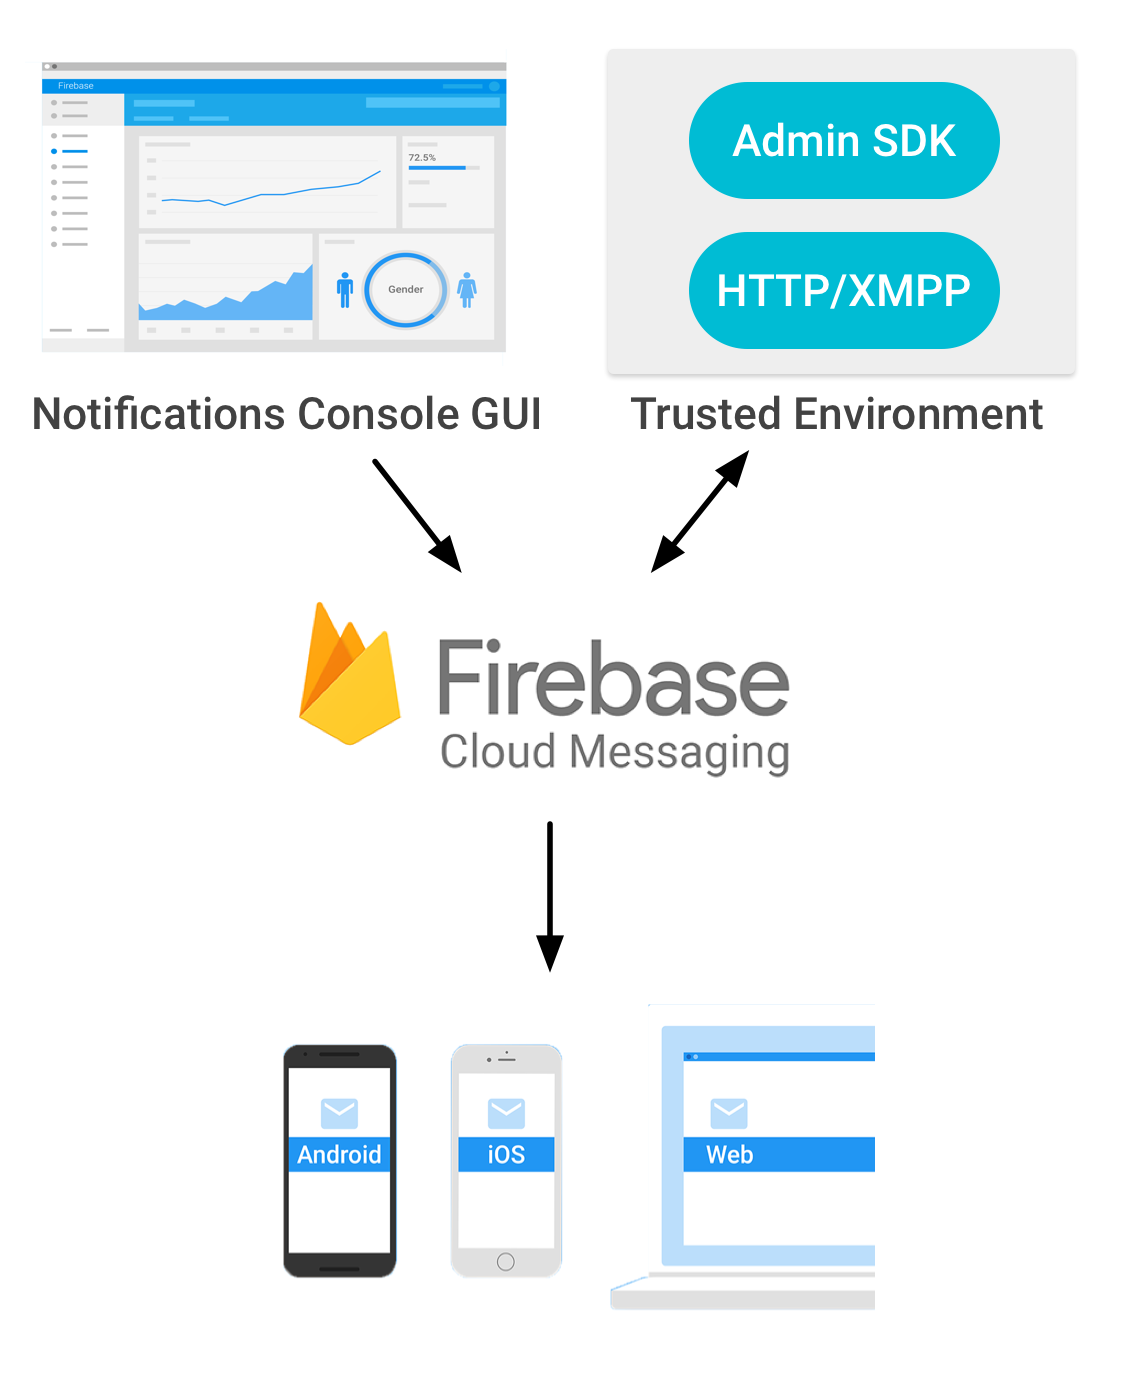
\includegraphics[width=0.5\linewidth]{messaging-overview}
	\caption[FCM messaging overview]{FCM messaging overview}
	\label{fig:messaging-overview}
\end{figure}

There are two main components:
\begin{itemize}
	\item A trusted environment such as an app server on which to build, target and send messages, and
	\item An iOS, Android, or Web (JavaScript) client app that receives messages
\end{itemize}
FCM basically allows server implementations to send out messages to single devices, groups or by topic. QuizFight uses only the former, since is simple and well suited for its purposes. This mode relies on installation tokens. At the very first installation a token is generated. This token is unique, but it may vary through the device's life. In fact, if the user reinstalls the app or if they performs a cache wipe, the token changes. This is why both at client and server side is required a mechanism to manage the token's life cycle. Further, different instances of the same app in different user's devices have different tokens associated to them. Hence, a notification has to be sent out to every different device, and different tokens have to be managed server side.

\subsection{Client side}
FCM requires two services running on the target device. They are used to check for token updates (remember a token is different after a cache wipe) and to be listening for new messages. Their declaration is shown in Listing~\ref{lst:fcmservices}.
\begin{lstlisting}[language=xml, caption={FCM Services}, label={lst:fcmservices}]
<service android:name=".services.CustomFirebaseInstanceID">
	<intent-filter>
		<action android:name="com.google.firebase.INSTANCE_ID_EVENT"/>
	</intent-filter>
</service>
<service android:name=".services.MessagingService">
	<intent-filter>
		<action android:name="com.google.firebase.MESSAGING_EVENT"/>
	</intent-filter>
</service>
\end{lstlisting}

\texttt{CustomFirebaseInstanceID} basically monitors token generation. As said, the registration token may change when:
\begin{itemize}
	\item the app deletes Instance ID;
	\item the app is restored on a new device;
	\item the user uninstalls/reinstalls the app;
	\item the user clears app data.
\end{itemize}
This Service overrides the method \texttt{onTokenRefresh()}. When a new token is available, it is sent to the server. QuizFight also sends \\\texttt{Settings.Secure.ANDROID\_ID}, in order to maintain the binding $<$device, token$>$. Even if the use of field is discouraged for most use cases, here it is necessary because we need to have the strong guarantee that a token must correspond to one device. Below are more details about that.

\texttt{MessagingService} is, on the other hand, used for receiving new messages. FCM provides two different message types: \textbf{notification} and \textbf{data}. The former can be sometimes thought of as ''display message''. FCM automatically displays the message to end-user devices on behalf of the client app. Notification messages have a predefined set of user-visible keys and an optional data payload of custom key-value pairs.In this case, if the app is not foreground, FCM provides the message to the system tray and no ''custom'' methods are invoked. This is why we rely only on data messages, handling both parsing and user notification by hand. We define a format for our messages, with both mandatory and Activity-dependent fields. Listing~\ref{lst:notification} shows the mandatory ones.
\begin{lstlisting}[language=json, caption={Mandatory fields for a notification}, label={lst:notification}]
{
	id: String,
	title: String,
	message: String
}
\end{lstlisting}
\texttt{id} is used to identify the notification type, and for opening the appropriate Activity at ''tap time''. \texttt{title} and \texttt{message} have the same meaning of the correspondent fields used in Android's notifications. Every \texttt{id} corresponds to a different triggered action, each of which requires specific parameters agreed with the server.

\subsection{Server side}
QuizFight's server is responsible for sending out notifications to clients. As we said, each app's instance is identified by using a unique token which life-cycle is managed by FCM. Nonetheless, we have to provide a way to handle token changes and multiple tokens for the same user. Fortunately, FCS allows us to send out almost 1000 messages at a time. We believe a user will not use more than 1000 devices with our application, so we consider this a safe bound.

Any time the token varies the client sends the new one to the server. It also sends \texttt{Settings.Secure.ANDROID\_ID}. Android discourages the use of such an identifier and recommends alternatives such as \textbf{Instance ID} or \textbf{globally unique ID} (GUID). Unfortunately those solutions are not suitable for our purposes. In fact, they provide a way to identify an application's \textit{instance}, but we already have something like that (i.e. FCM's tokens). Another solution could be the \textbf{Advertising IDs}, but they are user-resettable. This is why we had to rely on a non-resettable hardware identifier, such as \texttt{ANDROID\_ID}.

The client sends also the current logged user's username. Since users are identified using their Google Games' username, there is no other way to actually identify a user server-side. Then the server simply retrieves a document representing that user, looks for the actual device and substitutes the old token with the new one. In this way as soon as the token varies the server is notified by \texttt{CustomFirebaseInstanceID} and keeps everything up to date. Of course, if no device with the actual \texttt{ANDROID\_ID} is found a new device is added with the new token. From then on the new device will receive every notification.

When the server has to send out a new message it looks up users by their Google Games' username. It retrieves every device and every token (which is up to date by construction) and mails both the mandatory fields and the situation-dependent payload. We developed a module, \texttt{sendMessage}, which performs lookups and sending. Every message's information is directly provided by the REST service itself, so it is entirely a decentralized architecture without any dependency between the sending module and the information to be sent out.


